We now sketch some examples of data analytics tasks that Meteor provides support for. 

\subsection{Case Study: Top-K}

A top-K query is a common analytic query. For example, a cellular network operator may be interested in finding out the top-K applications users access on their mobile phones. Similarly, a search engine or CDN analyst will be interested in determining the top-K most visited URLs. 
A centralized algorithm for a top-K query will have to transfer all data to a central processing location and then aggregate, requiring a huge amount of bandwidth. For example, consider a network of 1000 cell towers, each connected to 50 mobile devices and generating a record for each device every two seconds. Each record has 200 fields, each field an integer value. The amount of data generated each minute over the network is therefore (1000 x 50 x 30 x 200 x 32) = 10 Gbits. Due to the sheer amount of data needed to be processed, it is much more preferable to process the data locally and do the aggregation only at the end. We plan to provide a top-k operator on top of Spark that implements the multi-round filtering approximate algorithm described in \cite{3}.

\subsection{Case Study: PageRank}

The PageRank algorithm is the cornerstone of Google’s search technology. It is used to rank the many trillions of URLs by importance. PageRank iteratively updates a rank for each webpage by adding up contributions from each page that links to it. On each iteration, the contribution of each page to its neighbors is r/n, where r is its rank, and n is the number of neighbors.
PageRank is an iterative algorithm as opposed to top-K, which is a one-time query. The most bandwidth-hungry stage during a MapReduce implementation of PageRank is the reduce step that aggregates the parent URL for a URL key to compute its rank. We plan to evaluate an approximation where this global reduce step is delayed and done locally instead. 

\subsection{Evaluation}

For our initial evaluation, we will use Emulab \cite{2}. Emulab is suitable since it gives us the ability to configure arbitrary network topologies and link bandwidths. For a start, each node in our Emulab topology will act as a datacenter and a link connecting two nodes will act as a link in the WAN. So far we have configured our environment in Emulab by installing Spark and its dependencies.

Our next steps are:
\begin{itemize}
\item Use Spark for the data analytics examples described above on an emulated distributed topology and show that as the available network bandwidth is reduced, job times increase.
\item Instrument Spark code to measure the bottleneck computations.
\item Implement the operators needed for our examples.
\end{itemize}

For a specific query, we envision our ‘money-graphs’ to be like this:

\begin{figure}[ht]
	\centering
	\begin{minipage}[b]{0.45\linewidth}
		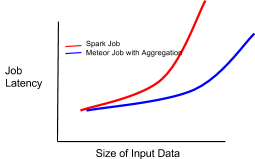
\includegraphics[width=2.3in]{fig_1.png}
		\caption{Latency}
		\label{fig:minipage1}
	\end{minipage}
	\quad
	\begin{minipage}[b]{0.45\linewidth}
		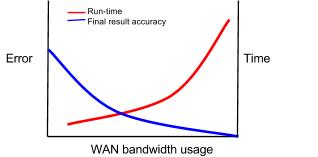
\includegraphics[width=2.6in]{fig_2.png}
		\caption{Error}
		\label{fig:minipage2}
	\end{minipage}
\end{figure}

\begin{comment}
\begin{figure}[ht!]
	\centering
	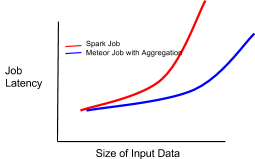
\includegraphics[width=2.4in]{fig_1.png}
	\caption{Latency}
	\label{overflow}
\end{figure}
\begin{figure}[ht!]
	\centering
	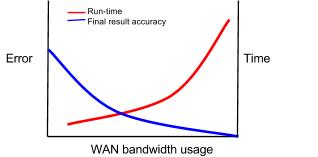
\includegraphics[width=2.6in]{fig_2.png}
	\caption{Error}
	\label{overflow}
\end{figure}
\end{comment}

Here we increase the size of the input data on the x-axis. A Spark job with no topological awareness starts taking longer and longer since the WAN link gets saturated. On the other hand, the corresponding Meteor job takes a lot less time since it uses aggregation to reduce the data needed to be sent over the WAN link. We plan to explore how modulating the bandwidth usage over WAN affects run-time as well as final result accuracy. We expect those result to be highly dependent on the application we are targeting.